% This work by Jeremy A. Hansen is licensed under a Creative Commons 
% Attribution-NonCommercial-ShareAlike 3.0 Unported License, 
% as described at http://creativecommons.org/licenses/by-nc-sa/3.0/legalcode

Up to this point, we have only discussed variables that are set up at compile time. 
Allocating space for variables at compile time is adequate in many cases, but occasionally a program will need to allocate space for data in memory while it is running. 
Consider the following code:

\noindent\begin{minipage}{\linewidth}\begin{lstlisting}
int arraySize;
cout << "Enter the number of elements in your array: ";
cin >> arraySize;
// We want to create an array with arraySize elements
int myArray[arraySize]; // SYNTAX ERROR!
\end{lstlisting}\end{minipage}

In order to allocate the space for \Code{myArray}, the compiler needs to know how many elements make up the array so that there is enough room in memory to accommodate the array. 
Unfortunately, the value of \Code{arraySize} is not known until the user enters something on the keyboard \emph{after the program has started running} and as a result, the compiler returns a syntax error. 

In C++, pointers are used to keep track of dynamically-allocated data:

\noindent\begin{minipage}{\linewidth}\begin{lstlisting}
float *fPtr = NULL; // (1) Declare a pointer to a float,
                    // which currently points nowhere
\end{lstlisting}\end{minipage}

In order to dynamically allocate an object of type \Code{float}, we use the \Code{new} operator: \nopagebreak[4]

\noindent\begin{minipage}{\linewidth}\begin{lstlisting}
fPtr = new float; // (2)
\end{lstlisting}\end{minipage}

\begin{figure}[tb]
  \centering
  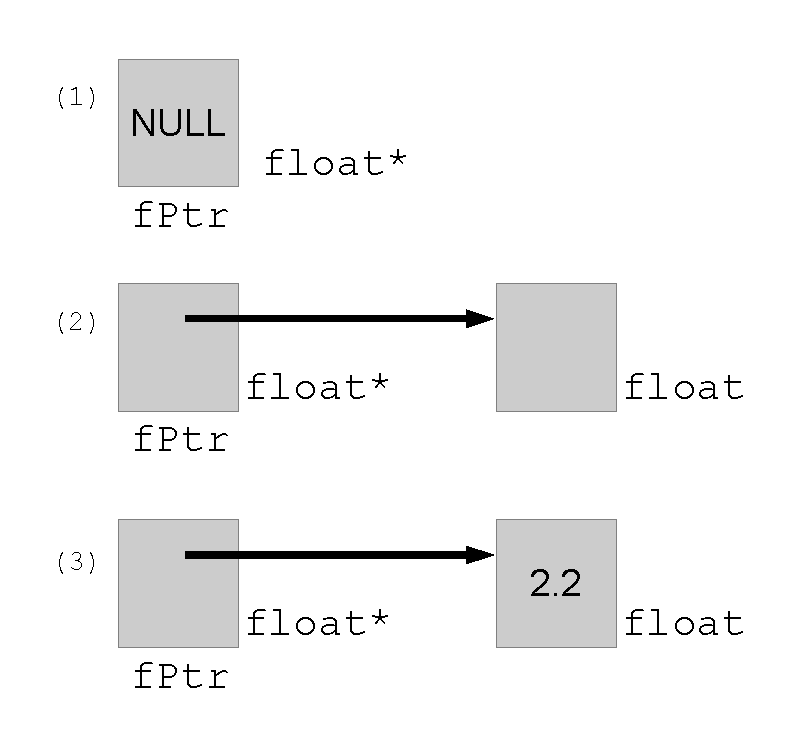
\includegraphics[width=0.7\textwidth]{diagrams/new_operator_diagram_1.pdf}
  \caption{Allocation and dereferencing of pointers} \label{fig:new_operator_diagram_1} 
\end{figure}

The created object of type \Code{float} does not have a name, so the \Code{new} operator returns a \Code{float*} that can be used to access the object. 
This pointer is stored in \Code{fPtr}. 
We use the dereference operator (\Code{*}, that is) to access the data:

\noindent\begin{minipage}{\linewidth}\begin{lstlisting}
*fPtr = 2.2; // (3) Goes to address at fPtr & puts 2.2 there
cout << "Data at " << fPtr << ": " << *fPtr << endl;
// This outputs: Data at 0x200102b0: 2.2
// Note that the address listed may differ
// Also note the difference between printing fPtr and *fPtr
\end{lstlisting}\end{minipage}

Notice that when a value is assigned to \Code{fPtr}, the pointer is being changed. 
When a value is assigned to \Code{*fPtr} (notice the dereference operator), the floating-point value at the address stored in \Code{fPtr} is changed. 

\begin{figure}[tbh]
  \centering
  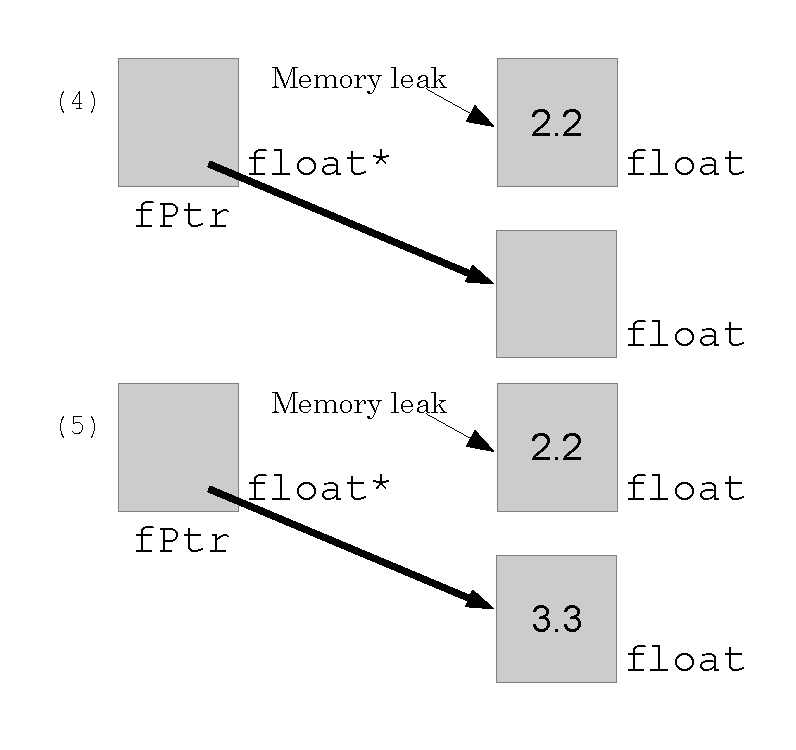
\includegraphics[width=0.7\textwidth]{diagrams/new_operator_diagram_2.pdf}
  \caption{Allocation and memory leaks} \label{fig:new_operator_diagram_2} 
\end{figure}

\noindent\begin{minipage}{\linewidth}\begin{lstlisting}
float *fPtr;
fPtr = new float;
*fPtr = 2.2; // Goes to address at fPtr & puts 2.2 there
cout << "Data at " << fPtr << ": " << *fPtr << endl;
fPtr = new float; // (4) fPtr now holds address of 
                  //     a new float object
*fPtr = 3.3; // (5)
cout << "Data now at " << fPtr << ": " << *fPtr << endl;
// This outputs: 
// Data at 0x200102b0: 2.2
// Data now at 0x200483c0: 3.3
\end{lstlisting}\end{minipage}

In this example, the \Code{float} containing the value $2.2$ still resides in memory, but is no longer reachable. 
This condition is called a \Keyword{memory leak}, and results in programs that consume more memory than they require. 
In order to free up the memory properly, we use the \Code{delete} operator: \nopagebreak[4]

\noindent\begin{minipage}{\linewidth}\begin{lstlisting}
float *fPtr;
fPtr = new float;
*fPtr = 2.2; // (6) Goes to the address at fPtr and stores 2.2 there
cout << "Data at " << fPtr << ": " << *fPtr << endl;
delete fPtr; // (7) Frees up the dynamically-allocated
             // memory at the address stored in fPtr
\end{lstlisting}\end{minipage}

At this point in the code, \Code{fPtr} can be referred to as a \Keyword{dangling pointer}, since the memory location it refers to is no longer valid, and the pointer just ``dangles'' there, pointing to nothing useful. 

\begin{figure}[tbh]
  \centering
  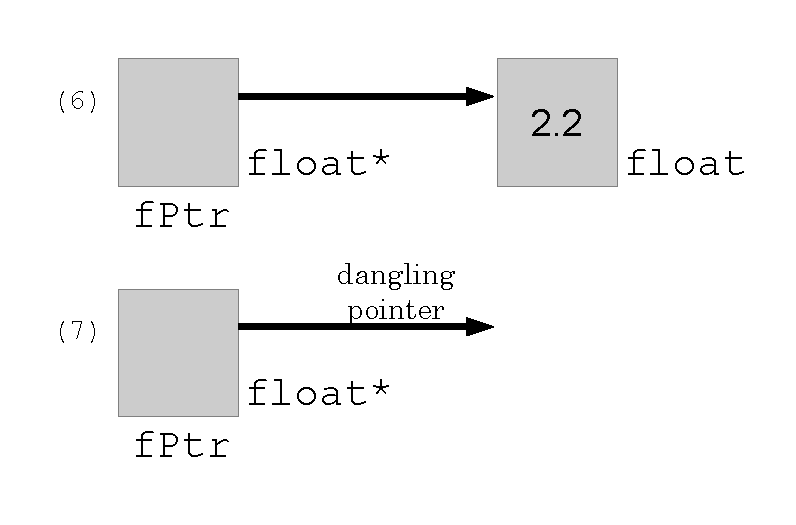
\includegraphics[width=0.7\textwidth]{diagrams/new_operator_diagram_3.pdf}
  \caption{Deallocation and dangling pointers} \label{fig:new_operator_diagram_3} 
\end{figure}
\noindent Arrays can be dynamically allocated, too:

\noindent\begin{minipage}{\linewidth}\begin{lstlisting}
float *fPtr = new float[10]; // Allocate an array of ten
              // floats and store their location in fPtr
\end{lstlisting}\end{minipage}

\noindent Arrays must be deleted in a similar fashion, but the syntax changes slightly:

\noindent\begin{minipage}{\linewidth}\begin{lstlisting}
delete [] fPtr; // Free up the entire array
\end{lstlisting}\end{minipage}


\LevelD{Review Questions}

\begin{enumerate}
	\item Write code to declare an integer pointer and dynamically allocate an integer. On the next line, assign this dynamically-allocated integer the value 13.

  \item Given the following code, write a few lines that deallocate any dynamically-allocated memory and set all pointer values to \Code{NULL}:

\noindent\begin{minipage}{\linewidth}\begin{lstlisting}
int *a = new int [24];
int *b;
int c;
b = &c;
\end{lstlisting}\end{minipage}


\end{enumerate}

\LevelD{Review Answers}

\begin{enumerate}
\item\noindent\begin{minipage}{\linewidth}\begin{lstlisting}
int *iPtr = new int;
*iPtr = 13;
\end{lstlisting}\end{minipage}

\item\noindent\begin{minipage}{\linewidth}\begin{lstlisting}
delete [] a;
a = NULL;
b = NULL;
\end{lstlisting}\end{minipage}

\end{enumerate}

\LevelD{Further Reading}

\begin{itemize}
\item \url{http://www.cplusplus.com/doc/tutorial/dynamic/}
\end{itemize}	

